% Isto é um exemplo de errata:


\begin{center}
	{\LARGE \textbf{Declaração de Atendimento às Observações da Banca}}
\end{center}
\vspace{\onelineskip}


Este exemplar foi revisado e alterado em relação à versão original, de acordo com as observações levantadas pela banca examinadora no dia da defesa, sob responsabilidade única do(a) autor(a) e com a anuência do(a) (co)orientador(a).
%
%Referente à dissertação de Mestrado intitulada “Simulações \textit{ab initio} de interfaces água/metal”, realizada por Graciele Martins Arvelos, fevereiro de 2023.
%
%Na folha 59, a Figura 13 corresponde a: 
%
%\begin{figure}[h!]
%	\centering
%	\caption{(a) Diferenças de densidades de carga $\Delta\rho$ das camadas H-Down, H-Up e H-Down/Up na superfície de tamanho $6\times4\times4$ e calculadas com os funcionais PBE e VDW-BH. Para todos os casos, o valor da isosuperfície foi $1.20 \times10^{-3}\;e/\AA$, onde vermelho (azul) indica uma diminuição (aumento) da densidade de carga durante a adsorção. (b) $ \Delta\rho $ médio ao longo do eixo z para os funcionais PBE (linha sólida) e VDW-BH (linha tracejada). As linhas pontilhadas correspondem às posições da última camada metálica de Pd e às posições dos átomos O e H das moléculas \textit{flat-down} e \textit{up} (funcional PBE). \label{fig:errata}}
%	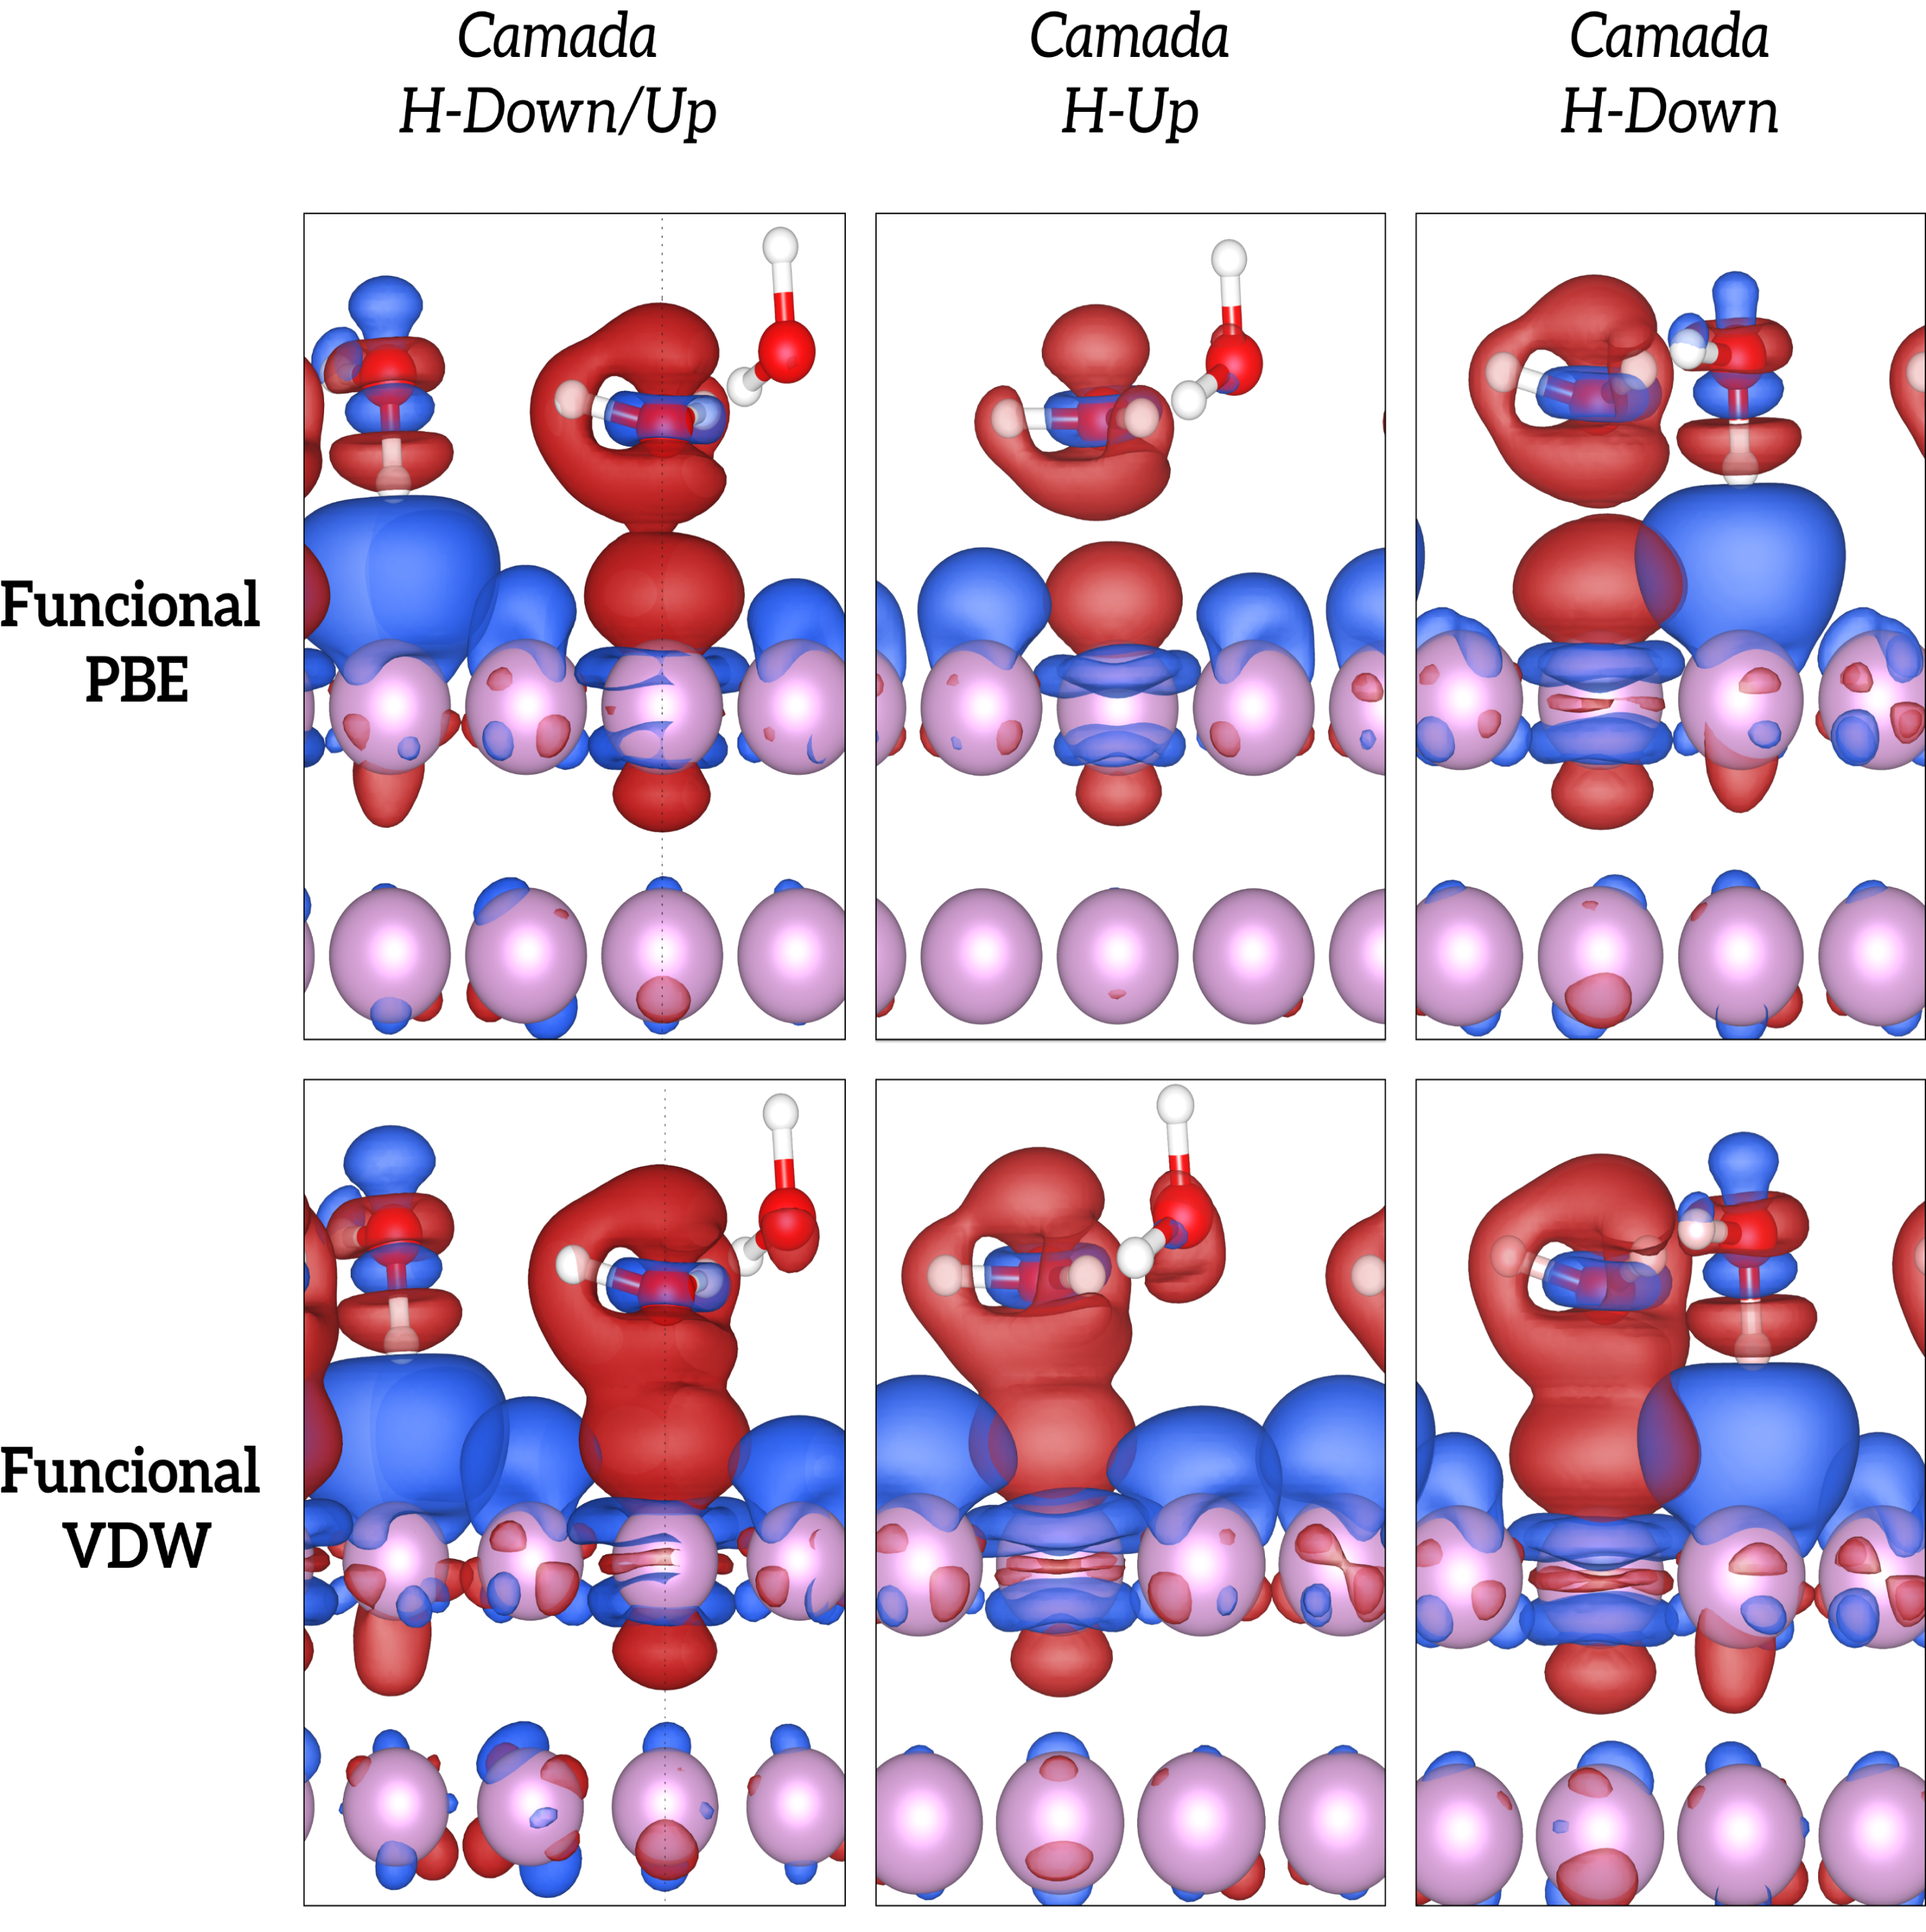
\includegraphics[scale=0.078]{figs/z_charge.png}
%	\legend{Fonte: Compilação da autora.}
%\end{figure}



 